% !TEX root = ../PDE4ML.tex

\section{A Primer on Optimal Transport}
\label{sec-primer-ot}

This primer fixes the optimal-transport notation used throughout the review. The goal is not to reproduce the full OT4ML development, but to keep the minimal objects needed for PDE methods: push-forward maps, Monge and Kantorovich formulations, Brenier maps, Wasserstein distances and displacement geodesics. The figures are used as a visual glossary: each one is placed next to the definition or theorem whose geometry it makes concrete.

\subsection{Measures and Push-Forwards}
\label{sec-measures}
\index{probability measure}
\index{push-forward}

Let $\X$ and $\Y$ be Polish metric spaces, meaning complete separable metric spaces. This assumption is the natural background for probability theory because it gives enough measurable structure for disintegration, weak convergence and compactness arguments while still covering Euclidean spaces, manifolds, discrete spaces and many path spaces.

\begin{defn}[Discrete measure]\label{def-discrete-measure}
	A discrete probability measure on $\X$ is
	\begin{equation}\label{eq-discr-meas}
		\alpha=\sum_{i=1}^n a_i\delta_{x_i},
		\qquad
		a_i\geq0,
		\qquad
		\sum_{i=1}^n a_i=1.
	\end{equation}
	If $a_i=1/n$, this is an empirical measure.
\end{defn}

\begin{defn}[Push-forward]\label{defn-pushfwd}
	Let $T:\X\to\Y$ be measurable and let $\alpha\in\Pp(\X)$. The push-forward $T_\sharp\alpha\in\Pp(\Y)$ is defined by
	\begin{equation}\label{eq-push-fwd}
		(T_\sharp\alpha)(B)=\alpha(T^{-1}(B))
	\end{equation}
	for all Borel sets $B\subset\Y$. Equivalently, for all bounded measurable $g:\Y\to\RR$,
	\begin{equation}\label{eq-equiv-pushfwd}
		\int_\Y g(y)\,\d(T_\sharp\alpha)(y)
		=
		\int_\X g(T(x))\,\d\alpha(x).
	\end{equation}
\end{defn}

If $X$ is a random variable with law $\alpha$, then $T_\sharp\alpha$ is the law of $T(X)$. This simple identity is the bridge between deterministic maps, particle systems and measure-valued PDEs.

\begin{prop}[Push-forward formula for densities]\label{prop-push-forward-densities}
	Let $\X=\Y=\RR^d$, let $T$ be a diffeomorphism, and let $\alpha=\rho_\alpha(x)\d x$. Then $\beta=T_\sharp\alpha$ has density
	\begin{equation}\label{eq-pfwd-density}
		\rho_\beta(y)
		=
		\rho_\alpha(T^{-1}(y))
		\left|\det \nabla T(T^{-1}(y))\right|^{-1}.
	\end{equation}
\end{prop}
\begin{proof}
	Apply the change-of-variables formula to~\eqref{eq-equiv-pushfwd}.
\end{proof}

Figure~\ref{fig:monge-jacobian-pushforward-density} makes the determinant factor visible. This is the first geometric warning behind transport PDEs: moving particles changes both their positions and the local volume element.

\begin{figure}[ht]
\centering
\setlength{\tabcolsep}{4pt}
\begin{tabular}{@{}cc@{}}

\includegraphics[width=.40\linewidth]{figures/monge-jacobian-pushforward-density/source-grid.pdf} &

\includegraphics[width=.40\linewidth]{figures/monge-jacobian-pushforward-density/target-density-grid.pdf} \\[-.1em]
\small uniform source grid &
\small pushed density and deformed grid
\end{tabular}
\caption{Jacobian determinant in the density push-forward formula. A smooth diffeomorphism compresses the middle of a colored square grid and applies a slight rotation. The source density is uniform, but the target density forms a central bump where deformed grid cells have smaller area. This is the geometric content of the factor $|\det\nabla T|^{-1}$ in~\eqref{eq-pfwd-density}, and later becomes the divergence structure of continuity equations.}
\label{fig:monge-jacobian-pushforward-density}
\end{figure}

\subsection{Monge Problems}
\label{sec-monge-formulation}
\label{sec-continuous-monge}
\index{Monge problem}

Monge's formulation asks for a deterministic map transporting one law onto another. It is geometrically direct and is the natural language for generative maps, but it is not convex and can be infeasible because maps cannot split mass.

\subsubsection{General Measures}

Given $\alpha\in\Pp(\X)$, $\beta\in\Pp(\Y)$ and a cost $c:\X\times\Y\to\RR_+$, the Monge problem is
\begin{equation}\label{eq-monge-continuous}
	\Monge_c(\alpha,\beta)
	\eqdef
	\inf_T
	\left\{
		\int_\X c(x,T(x))\,\d\alpha(x)
		\; ; \;
		T_\sharp\alpha=\beta
	\right\}.
\end{equation}
The constraint $T_\sharp\alpha=\beta$ means that the endpoint law is imposed exactly. If $\alpha=\delta_x$ and $\beta$ is not a Dirac mass, the feasible set is empty; this is the simplest mass-splitting obstruction.

\begin{prop}[Existence of transport maps from atomless sources]\label{prop-existence-transport-map-atomless}
	Let $\alpha$ and $\beta$ be Borel probability measures on Polish spaces, and assume that $\alpha$ is atomless. Then there exists a measurable map $T$ such that $T_\sharp\alpha=\beta$.
\end{prop}
\begin{proof}
	Use a standard measure-isomorphism theorem to identify the atomless probability space generated by $\alpha$ with Lebesgue measure on $[0,1]$, modulo null sets. A generalized quantile map sends Lebesgue measure on $[0,1]$ to $\beta$ after a Borel parametrization of the target space. Composing both maps gives a transport map.
\end{proof}

A useful asymmetric case is semi-discrete transport: the source has a density, the target is finitely supported, and a Monge map partitions space into cells. Figure~\ref{fig:monge-semidiscrete-maps} gives the cell picture before the fully discrete assignment problem. It also explains why reversing source and target would usually be impossible: finitely many source atoms cannot be mapped deterministically onto a continuous density.

\begin{figure}[ht]
\centering
\begin{tabular}{@{}cc@{}}
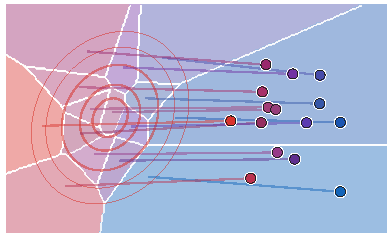
\includegraphics[width=.48\linewidth]{figures/monge-semidiscrete-maps/gaussian-to-discrete.pdf} &
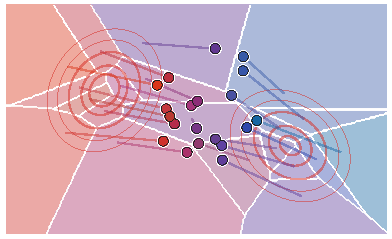
\includegraphics[width=.48\linewidth]{figures/monge-semidiscrete-maps/mixture-to-discrete.pdf} \\[-.1em]
\small Gaussian source to 15 atoms &
\small two-mode source to 20 atoms
\end{tabular}
\caption{Semi-discrete Monge maps. The red contours show the continuous source density. The colored regions are numerical Laguerre cells with approximately equal source mass, and the circular atoms form the discrete target. Faint segments connect cell barycenters to their images under the piecewise-constant Monge map, making the map-as-partition viewpoint explicit.}
\label{fig:monge-semidiscrete-maps}
\end{figure}

\subsubsection{Discrete Monge Problem}
\label{sec-monge-pbm}
\index{assignment problem}

For equal-size empirical measures
\[
	\alpha=\frac1n\sum_{i=1}^n\delta_{x_i},
	\qquad
	\beta=\frac1n\sum_{j=1}^n\delta_{y_j},
\]
and distinct target points, a feasible Monge map is a permutation. The discrete problem is therefore the assignment problem
\begin{equation}\label{eq-optimal-assignment}
	\min_{\sigma\in\Perm(n)}
	\frac1n\sum_{i=1}^n C_{i,\sigma(i)},
	\qquad
	C_{ij}=c(x_i,y_j).
\end{equation}

\begin{prop}[Empirical Monge maps and matchings]\label{prop-empirical-monge-matching}
	Assume that the source atoms $x_i$ are distinct and that $\alpha=n^{-1}\sum_i\delta_{x_i}$, $\beta=n^{-1}\sum_j\delta_{y_j}$. If the $y_j$ are distinct and $T_\sharp\alpha=\beta$, then there exists $\sigma\in\Perm(n)$ such that $T(x_i)=y_{\sigma(i)}$ for all $i$.
\end{prop}
\begin{proof}
	For any target atom $z$, the identity $T_\sharp\alpha=\beta$ gives
	\[
		\beta(\{z\})=\alpha(T^{-1}(\{z\}))
		=
		\frac1n\#\{i:T(x_i)=z\}.
	\]
	Each target atom has mass $1/n$, so it receives exactly one source atom.
\end{proof}

In one dimension, convex costs have a special monotonicity structure: after sorting the source and target points, the equal-rank matching is optimal. This order structure is exceptional and does not survive in higher-dimensional point clouds.

The next two figures isolate the role of order on the line. Figure~\ref{fig:matching-1d-quantile-assignment} shows equal-rank matching for convex costs, while Figure~\ref{fig:matching-1d-convex-concave-costs} contrasts it with a concave-cost regime where crossings become favorable.

\begin{figure}[ht]
\centering
\begin{tabular}{@{}cc@{}}
\small two mixtures & \small one mode to three modes \\[-.15em]
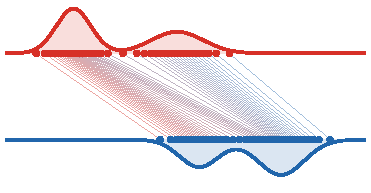
\includegraphics[width=.46\linewidth]{figures/matching-1d-quantile-assignment/quantile-assignment.pdf} &
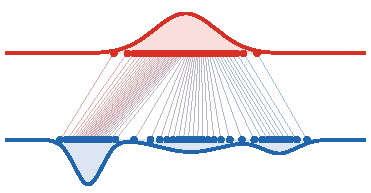
\includegraphics[width=.46\linewidth]{figures/matching-1d-quantile-assignment/central-to-three-modes.pdf}
\end{tabular}
\caption{One-dimensional optimal matching by quantile sorting. The red and blue curves are smooth laws used to generate equal-weight empirical measures; the dots are inverse-CDF samples at common quantile levels. For convex costs on the line, the monotone assignment connects equal ranks.}
\label{fig:matching-1d-quantile-assignment}
\end{figure}

\begin{figure}[ht]
\centering
\begin{tabular}{@{}cc@{}}
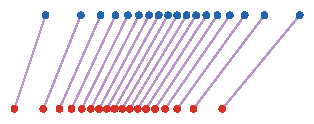
\includegraphics[width=.46\linewidth]{figures/matching-1d-convex-concave-costs/convex.pdf} &
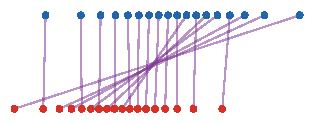
\includegraphics[width=.46\linewidth]{figures/matching-1d-convex-concave-costs/concave.pdf} \\[-.1em]
\small convex cost, $p=2$ &
\small concave cost, $p=1/2$ \\[.25em]

\includegraphics[width=.46\linewidth]{figures/matching-1d-convex-concave-costs/mixture-convex.pdf} &

\includegraphics[width=.46\linewidth]{figures/matching-1d-convex-concave-costs/mixture-concave.pdf} \\[-.1em]
\small two-mode to three-mode, $p=2$ &
\small two-mode to three-mode, $p=1/2$
\end{tabular}
\caption{One-dimensional assignments for costs $c_p(x,y)=|x-y|^p$. For the convex quadratic cost, equal ranks are matched and the segments do not cross. For the concave cost, the optimum creates long crossing exchanges. Thus monotone rearrangement is a convex-cost phenomenon, not a generic property of all transport costs.}
\label{fig:matching-1d-convex-concave-costs}
\end{figure}

The line also has a useful periodic variant. On the circle, one first chooses a cut, unfolds both measures into an interval and then applies the monotone one-dimensional assignment. Optimizing over the cut restores the circular geometry; see Figure~\ref{fig:monge-circle-cut-unfolding}. This is still an ordered one-dimensional construction, but the order is cyclic rather than linear.

\begin{figure}[ht]
\centering
\begin{tabular}{@{}cc@{}}
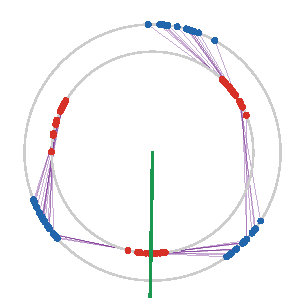
\includegraphics[width=.32\linewidth]{figures/monge-circle-cut-unfolding/circle.pdf} &
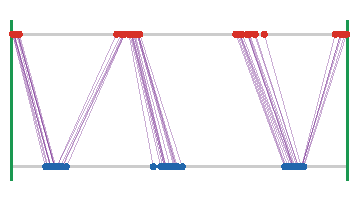
\includegraphics[width=.54\linewidth]{figures/monge-circle-cut-unfolding/unfolded.pdf} \\[-.1em]
\small circular matching &
\small unfolded interval
\end{tabular}
\caption{Optimal transport on the circle by cutting and unfolding. Red and blue atoms live on two copies of the circle, purple segments show the optimal cyclic matching, and the green radius marks the chosen cut. Once the circle is opened at this angle, the same assignment becomes a monotone one-dimensional matching on the interval.}
\label{fig:monge-circle-cut-unfolding}
\end{figure}

In two dimensions there is no global sorting rule. Figure~\ref{fig:matching-2d-cost-exponent} keeps the same two point clouds and changes only the exponent in the cost, showing that the optimal permutation is already a genuinely geometric object.

\begin{figure}[ht]
\centering
\begin{tabular}{@{}cccc@{}}

\includegraphics[width=.225\linewidth]{figures/matching-2d-cost-exponent/p0p5.pdf} &

\includegraphics[width=.225\linewidth]{figures/matching-2d-cost-exponent/p1.pdf} &

\includegraphics[width=.225\linewidth]{figures/matching-2d-cost-exponent/p2.pdf} &

\includegraphics[width=.225\linewidth]{figures/matching-2d-cost-exponent/p6.pdf} \\[-.1em]
\small $\norm{x-y}^{1/2}$ &
\small $\norm{x-y}$ &
\small $\norm{x-y}^2$ &
\small $\norm{x-y}^6$
\end{tabular}
\caption{Optimal assignments between the same two planar point clouds for four powers of the Euclidean distance. The feasible permutations are unchanged, but the selected matching changes with the cost geometry: small powers tolerate long exchanges, whereas larger powers suppress the longest edges.}
\label{fig:matching-2d-cost-exponent}
\end{figure}

The permutation viewpoint also assumes equal cardinalities and equal weights. Figure~\ref{fig:matching-resolution-and-weights} previews the Kantorovich matrix formulation: as soon as masses or resolutions differ, transport must allow splitting and merging.

\begin{figure}[ht]
\centering
\begin{tabular}{ccc}

\includegraphics[width=.30\linewidth]{figures/matching-resolution-and-weights/balanced.pdf} &
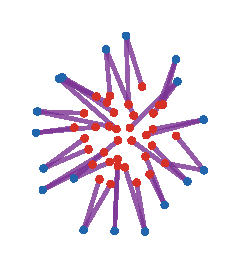
\includegraphics[width=.30\linewidth]{figures/matching-resolution-and-weights/rectangular.pdf} &
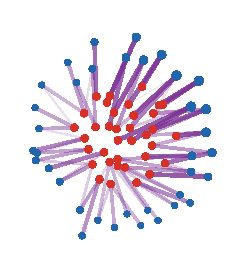
\includegraphics[width=.30\linewidth]{figures/matching-resolution-and-weights/weighted.pdf} \\[-.1em]
\small $n=m$ &
\small $m<n$ &
\small nonuniform target weights
\end{tabular}
\caption{From assignments to transport plans, using the same disk-to-annulus geometry as Figure~\ref{fig:matching-2d-cost-exponent}. In the balanced equal-weight case, each source atom is matched to one target atom. With fewer target atoms, or with strongly nonuniform target weights, the coupling must merge or split mass; segment thickness and opacity encode transported mass.}
\label{fig:matching-resolution-and-weights}
\end{figure}

Rational weights give a precise bridge between assignments and transport matrices. If $a_i=k_i/N$ and $b_j=\ell_j/N$, one may duplicate $x_i$ exactly $k_i$ times and $y_j$ exactly $\ell_j$ times, solve a uniform assignment with $N$ particles on each side, and collapse the result back to the original supports. Figure~\ref{fig:matching-rational-duplication} shows how repeated duplicated matches appear as several transport segments attached to the same displayed atom.

\begin{figure}[ht]
\centering
\begin{tabular}{@{}ccc@{}}
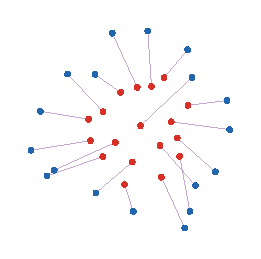
\includegraphics[width=.29\linewidth]{figures/matching-rational-duplication/uniform.pdf} &
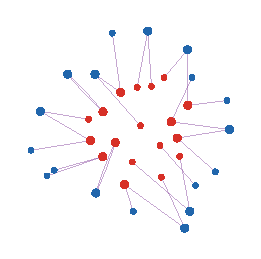
\includegraphics[width=.29\linewidth]{figures/matching-rational-duplication/binary.pdf} &
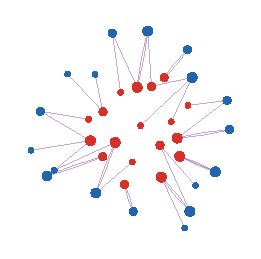
\includegraphics[width=.29\linewidth]{figures/matching-rational-duplication/ternary.pdf} \\[-.1em]
\small uniform multiplicities &
\small binary multiplicities &
\small ternary multiplicities
\end{tabular}
\caption{Rational weights as duplicated uniform matchings. The red and blue locations are displayed once, while disk areas encode integer multiplicities. After duplication, the uniform assignment may contain several matched copies of the same displayed point; collapsing these copies gives the integer count matrix underlying a rational-weight Kantorovich plan.}
\label{fig:matching-rational-duplication}
\end{figure}

\subsection{Kantorovich Problems}
\label{sec-kantorovich}
\index{Kantorovich problem}
\index{coupling}

Kantorovich's relaxation replaces deterministic maps by joint probability measures. It is the convex formulation used throughout the rest of the review, and it is the object whose dynamic counterpart becomes the Benamou--Brenier PDE.

\subsubsection{General Measures}
\label{sec-kantorovich-continuous}

\begin{defn}[Marginals of a joint measure]\label{def-joint-marginals}
	Let $\pi\in\Pp(\X\times\Y)$ and let $P_\X(x,y)=x$, $P_\Y(x,y)=y$. Its marginals are $(P_\X)_\sharp\pi$ and $(P_\Y)_\sharp\pi$.
\end{defn}

\begin{defn}[Couplings]\label{def-continuous-couplings}
	The set of couplings between $\alpha\in\Pp(\X)$ and $\beta\in\Pp(\Y)$ is
	\begin{equation}\label{eq-coupling-generic}
		\Couplings(\alpha,\beta)
		\eqdef
		\{\pi\in\Pp(\X\times\Y)\; ;\; (P_\X)_\sharp\pi=\alpha,\ (P_\Y)_\sharp\pi=\beta\}.
	\end{equation}
\end{defn}

The set is never empty, since it contains the tensor product $\alpha\otimes\beta$. The Kantorovich problem is
\begin{equation}\label{eq-mk-generic}
	\MK_c(\alpha,\beta)
	\eqdef
	\inf_{\pi\in\Couplings(\alpha,\beta)}
	\int_{\X\times\Y} c(x,y)\,\d\pi(x,y).
\end{equation}
If $T_\sharp\alpha=\beta$, then $\pi=(\Id,T)_\sharp\alpha$ is a coupling, so Kantorovich is a relaxation of Monge.

Figure~\ref{fig:kantorovich-coupling-polylines} gives a first visual dictionary for couplings: a graph coupling is deterministic, the tensor product is independent and diffuse, and an optimal relaxed plan selects the dependence that lowers the cost. This is the finite-dimensional picture to keep in mind when the same symbol $\pi$ later denotes a dynamic plan or a law on paths.

\begin{figure}[ht]
\centering
\begin{tabular}{@{}ccc@{}}
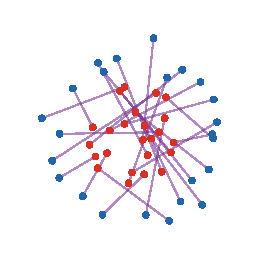
\includegraphics[width=.28\linewidth]{figures/kantorovich-coupling-polylines/graph.pdf} &
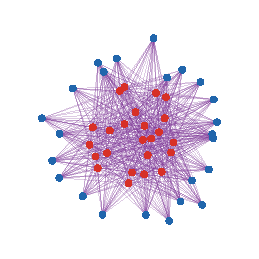
\includegraphics[width=.28\linewidth]{figures/kantorovich-coupling-polylines/product.pdf} &
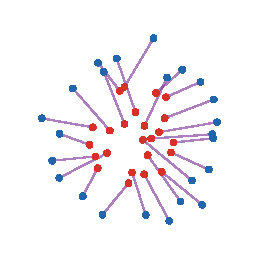
\includegraphics[width=.28\linewidth]{figures/kantorovich-coupling-polylines/optimal.pdf} \\[-.1em]
\small deterministic graph & \small product plan $\alpha\otimes\beta$ & \small optimal plan
\end{tabular}
\caption{Discrete couplings represented as straight transport segments. A deterministic graph coupling sends each source to one destination, the product plan spreads every source mass over all targets, and the optimal Kantorovich plan minimizes the quadratic cost while being allowed to split mass. Line width and opacity encode the transported mass.}
\label{fig:kantorovich-coupling-polylines}
\end{figure}

\begin{prop}[Existence on compact spaces]\label{prop-kantorovich-existence-compact}
	If $\X$ and $\Y$ are compact metric spaces and $c$ is continuous, then the infimum in~\eqref{eq-mk-generic} is attained.
\end{prop}
\begin{proof}
	The set $\Couplings(\alpha,\beta)$ is tight and closed for weak convergence, hence compact. The functional $\pi\mapsto\int c\,\d\pi$ is continuous on this compact set.
\end{proof}

\subsubsection{Discrete Kantorovich Problem}
\label{sec-discrete-relaxation}

For discrete measures $\alpha=\sum_i a_i\delta_{x_i}$ and $\beta=\sum_j b_j\delta_{y_j}$, a coupling is a nonnegative matrix with prescribed row and column sums.

\begin{defn}[Discrete couplings and mass conservation]\label{def-discrete-couplings}
	For weights $\a\in\simplex_n$ and $\b\in\simplex_m$,
	\begin{equation}\label{eq-discr-couplings}
		\CouplingsD(\a,\b)
		\eqdef
		\left\{
		\P\in\RR_+^{n\times m}
		\; ; \;
		\P\ones_m=\a,\ \P^\top\ones_n=\b
		\right\}.
	\end{equation}
\end{defn}

\begin{defn}[Discrete product coupling]\label{def-discrete-product-coupling}
	The product, or trivial, coupling is $(\a\otimes\b)_{ij}=a_i b_j$.
\end{defn}

Given $C_{ij}=c(x_i,y_j)$, the discrete Kantorovich value is the linear program
\begin{equation}\label{eq-kanto-discr}
	\MKD_\C(\a,\b)
	\eqdef
	\min_{\P\in\CouplingsD(\a,\b)}
	\sum_{i,j} C_{ij}P_{ij}.
\end{equation}
When $m=n$ and $\a=\b=\ones_n/n$, the Birkhoff--von Neumann theorem implies that this relaxation admits an optimal permutation plan, so it is tight for the balanced assignment problem. For nonuniform weights or unequal cardinalities, mass splitting is essential.

The Birkhoff theorem is also a useful mental model for linear programming over couplings: a bistochastic matrix can be moved along cycles in its positive-support bipartite graph until a permutation component is exposed. Figure~\ref{fig:birkhoff-von-neumann-cycle} displays this cycle mechanism in the finite case.

\begin{figure}[ht]
\centering
\begin{tabular}{@{}cc@{}}
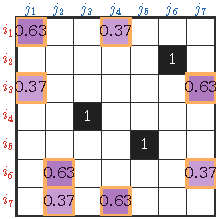
\includegraphics[width=.34\linewidth]{figures/birkhoff-von-neumann-cycle/matrix.pdf} &
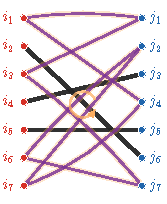
\includegraphics[width=.40\linewidth]{figures/birkhoff-von-neumann-cycle/support-graph.pdf} \\[-.1em]
\small bistochastic matrix &
\small support graph and cycle
\end{tabular}
\caption{Cycle certificate in the Birkhoff--von Neumann proof. The matrix is bistochastic but not a permutation matrix. Its positive support defines a bipartite graph; a fractional cycle permits an alternating add-subtract perturbation that preserves row and column sums and pushes at least one entry to zero. Repeating this exposes permutation matrices as extreme points.}
\label{fig:birkhoff-von-neumann-cycle}
\end{figure}

Two complementary pictures of the discrete relaxation are useful. Figure~\ref{fig:kantorovich-permutation-versus-splitting} keeps the physical segments visible, while Figure~\ref{fig:kantorovich-coupling-matrix-marginals} shows the same idea as a matrix with prescribed row and column sums.

\begin{figure}[ht]
\centering
\begin{tabular}{@{}cccc@{}}
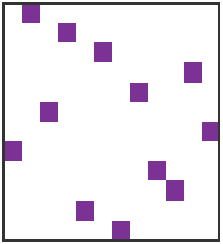
\includegraphics[width=.18\linewidth]{figures/kantorovich-permutation-versus-splitting/permutation-matrix.pdf} &
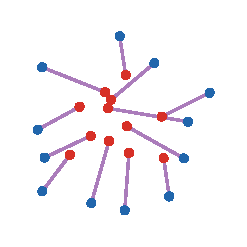
\includegraphics[width=.23\linewidth]{figures/kantorovich-permutation-versus-splitting/permutation-transport.pdf} &
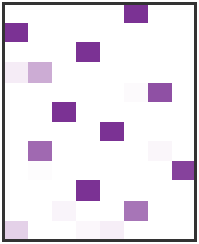
\includegraphics[width=.16\linewidth]{figures/kantorovich-permutation-versus-splitting/splitting-matrix.pdf} &
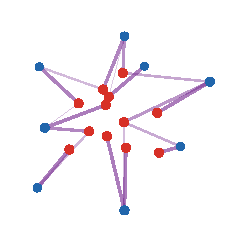
\includegraphics[width=.23\linewidth]{figures/kantorovich-permutation-versus-splitting/splitting-transport.pdf} \\[-.1em]
\small permutation matrix &
\small assignment segments &
\small splitting matrix &
\small splitting segments
\end{tabular}
\caption{From permutation matrices to splitting couplings. When two empirical measures have the same number of atoms and uniform weights, an optimal plan can be a permutation matrix. Once target masses are nonuniform, admissible couplings may split one source among several targets or merge several sources into one target.}
\label{fig:kantorovich-permutation-versus-splitting}
\end{figure}

\begin{figure}[ht]
\centering
\begin{tabular}{@{}cccc@{}}
\small product, 20 bins & \small OT, 20 bins & \small product, 200 bins & \small OT, 200 bins \\[-.15em]
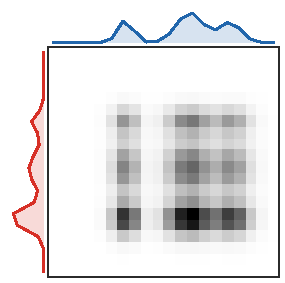
\includegraphics[width=.22\linewidth]{figures/kantorovich-coupling-matrix-marginals/product-20.pdf} &
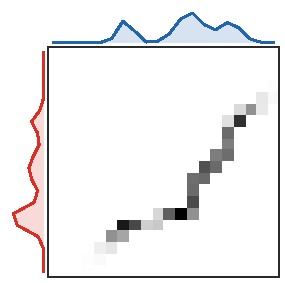
\includegraphics[width=.22\linewidth]{figures/kantorovich-coupling-matrix-marginals/optimal-20.pdf} &
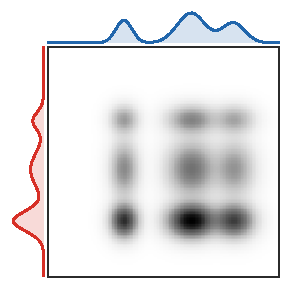
\includegraphics[width=.22\linewidth]{figures/kantorovich-coupling-matrix-marginals/product-200.pdf} &
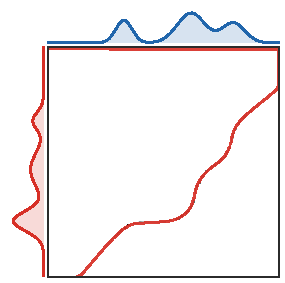
\includegraphics[width=.22\linewidth]{figures/kantorovich-coupling-matrix-marginals/optimal-200.pdf}
\end{tabular}
\caption{Coupling matrices with their prescribed marginals. The central grayscale image displays $P_{ij}$; the red curve on the left is the source marginal $a$, and the blue curve on top is the target marginal $b$. The independent product plan is diffuse, whereas the one-dimensional optimal plan concentrates near the monotone quantile correspondence.}
\label{fig:kantorovich-coupling-matrix-marginals}
\end{figure}

\subsection{Brenier Maps and Quadratic OT}
\label{sec-monge-existence-uniqueness}
\index{Brenier theorem}
\index{quadratic cost}

The quadratic Euclidean cost is the central case for Wasserstein PDEs. Brenier's theorem says that the optimal coupling is induced by a gradient of a convex potential whenever the source is sufficiently diffuse.

\begin{thm}[Brenier]\label{thm-brenier}
	Let $\alpha,\beta\in\Pp_2(\RR^d)$ and assume that $\alpha$ is absolutely continuous with respect to Lebesgue measure. For the cost $c(x,y)=\norm{x-y}^2$, there exists a convex function $\phi$ such that
	\[
		T=\nabla\phi,
		\qquad
		T_\sharp\alpha=\beta,
	\]
	and $T$ is the unique optimal Monge map $\alpha$-almost everywhere. The associated optimal Kantorovich plan is unique and equals $(\Id,T)_\sharp\alpha$.
\end{thm}

Thus quadratic OT is not merely a linear program over couplings; under absolute continuity it is a nonlinear elliptic problem for a convex potential. When $\alpha=\rho_\alpha\d x$ and $\beta=\rho_\beta\d y$ are smooth positive densities and $T=\nabla\phi$ is smooth, the change-of-variables formula gives the Monge--Amp\`ere equation
\begin{equation}\label{eq-monge-ampere}
	\rho_\alpha(x)
	=
		\rho_\beta(\nabla\phi(x))\det(\nabla^2\phi(x)).
\end{equation}

Figure~\ref{fig:monge-caffarelli-nonconvex-map} should be read as a geometric stress test rather than a regularity theorem. It displays the particle interpolation induced by a quadratic assignment from a convex disk to a connected nonconvex target, making visible why regularity assumptions on the target geometry matter.

\begin{figure}[ht]
\centering
\setlength{\tabcolsep}{1.5pt}
\begin{tabular}{@{}ccccc@{}}
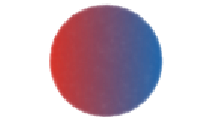
\includegraphics[width=.19\linewidth]{figures/monge-caffarelli-nonconvex-map/mccann-t000.pdf} &
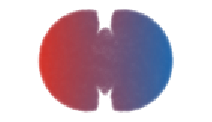
\includegraphics[width=.19\linewidth]{figures/monge-caffarelli-nonconvex-map/mccann-t025.pdf} &
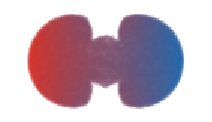
\includegraphics[width=.19\linewidth]{figures/monge-caffarelli-nonconvex-map/mccann-t050.pdf} &
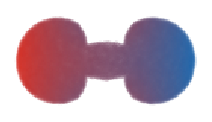
\includegraphics[width=.19\linewidth]{figures/monge-caffarelli-nonconvex-map/mccann-t075.pdf} &

\includegraphics[width=.19\linewidth]{figures/monge-caffarelli-nonconvex-map/mccann-t100.pdf} \\[-.1em]
\small $t=0$ &
\small $t=1/4$ &
\small $t=1/2$ &
\small $t=3/4$ &
\small $t=1$
\end{tabular}
\caption{Empirical quadratic OT interpolation from a disk to a connected nonconvex two-disk domain. A dense farthest-point sample of the disk is matched to a dense farthest-point sample of two disks connected by a thin rectangle. The panels display $(1-t)x_i+tT_N(x_i)$ for the empirical optimal assignment $T_N$; colors are inherited from the horizontal coordinate of $x_i$ in the initial disk, so transported material regions can be tracked.}
\label{fig:monge-caffarelli-nonconvex-map}
\end{figure}

The Gaussian case is the main closed-form model reused later for Gaussian closures of flows.

\begin{prop}[Gaussian $\Wass_2$ formula and Bures covariance term]\label{prop-gaussian-w2-bures}
	Let $\alpha=\Gaussian(m_\alpha,\Sigma_\alpha)$ and $\beta=\Gaussian(m_\beta,\Sigma_\beta)$ with positive definite covariance matrices. Then the quadratic optimal map is affine,
	\[
		T(x)=m_\beta+A(x-m_\alpha),
		\qquad
		A=\Sigma_\alpha^{-1/2}
		(\Sigma_\alpha^{1/2}\Sigma_\beta\Sigma_\alpha^{1/2})^{1/2}
		\Sigma_\alpha^{-1/2},
	\]
	and
	\begin{equation}\label{eq-dist-gauss}
		\Wass_2^2(\alpha,\beta)
		=
		\norm{m_\alpha-m_\beta}^2
		+
		\tr\left(
			\Sigma_\alpha+\Sigma_\beta
			-2(\Sigma_\alpha^{1/2}\Sigma_\beta\Sigma_\alpha^{1/2})^{1/2}
		\right).
	\end{equation}
\end{prop}
\begin{proof}
	The affine map above sends the first Gaussian to the second and has symmetric positive definite linear part. It is therefore the gradient of a convex quadratic potential, so Brenier's theorem gives optimality. Substituting the affine displacement in the quadratic transport cost gives the formula.
\end{proof}

Figure~\ref{fig:monge-gaussian-w2-geodesic} turns the closed form into three complementary pictures: densities in one dimension, covariance ellipses in two dimensions, and a curve inside the cone of positive semidefinite matrices.

\begin{figure}[ht]
\centering
\begin{tabular}{@{}ccc@{}}

\includegraphics[width=.31\linewidth]{figures/monge-gaussian-w2-geodesic/densities-1d-a.pdf} &

\includegraphics[width=.31\linewidth]{figures/monge-gaussian-w2-geodesic/ellipses-rotated-anisotropic.pdf} &

\includegraphics[width=.31\linewidth]{figures/monge-gaussian-w2-geodesic/cone-2d.pdf} \\[-.1em]
\small one-dimensional densities &
\small covariance ellipses &
\small covariance cone
\end{tabular}
\caption{Gaussian $\Wass_2$ geodesics. In one dimension, the mean and standard deviation interpolate linearly. In two dimensions, the affine Brenier map transports covariance ellipses along the Bures covariance geometry appearing in~\eqref{eq-dist-gauss}. The cone panel represents $2\times2$ positive semidefinite covariances and shows that covariance interpolation is not generally Euclidean in matrix entries.}
\label{fig:monge-gaussian-w2-geodesic}
\end{figure}

\subsection{Wasserstein Distances and Geodesics}
\label{sec-kantorovich-metric}
\index{Wasserstein distance}
\index{Wasserstein geodesic}

The metric structure used in the PDE sections is obtained by taking the $p$-th root of the Kantorovich cost for a ground metric.

\begin{defn}[Wasserstein distance]\label{def-wasserstein-distance}
	Let $(\X,d)$ be a metric space and $p\geq1$. For $\alpha,\beta\in\Pp_p(\X)$,
	\begin{equation}\label{eq-defn-wass-dist}
		\Wass_p(\alpha,\beta)
		\eqdef
		\left(
		\inf_{\pi\in\Couplings(\alpha,\beta)}
		\int_{\X\times\X} d(x,y)^p\,\d\pi(x,y)
		\right)^{1/p}.
	\end{equation}
\end{defn}

\begin{prop}[Metric property of the Wasserstein distance]\label{prop-metric-measure}
	If $(\X,d)$ is a metric space, then $\Wass_p$ is a distance on $\Pp_p(\X)$.
\end{prop}
\begin{proof}
	Nonnegativity and symmetry are immediate. If $\Wass_p(\alpha,\beta)=0$, the optimal mass can only lie on the diagonal, hence $\alpha=\beta$. The triangle inequality follows from the gluing lemma: glue an optimal coupling between $\alpha$ and $\beta$ with one between $\beta$ and $\gamma$ to obtain a joint law of $(X,Y,Z)$; then apply Minkowski's inequality to $d(X,Z)\leq d(X,Y)+d(Y,Z)$.
\end{proof}

The gluing step is abstract but elementary in the discrete case. If $P\in\CouplingsD(\a,\b)$ and $Q\in\CouplingsD(\b,\VectMode{c})$, then
\[
	R=P\diag(\b)^{-1}Q
\]
is a feasible coupling between $\a$ and $\VectMode{c}$ whenever all entries of $\b$ are positive. Figure~\ref{fig:kantorovich-discrete-gluing-lemma} visualizes this composition of plans through an intermediate marginal.

\begin{figure}[ht]
\centering
\begin{tabular}{@{}cccc@{}}
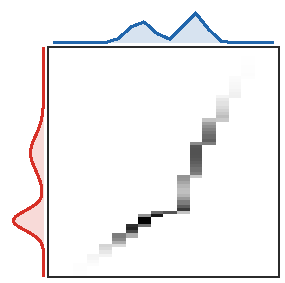
\includegraphics[width=.22\linewidth]{figures/kantorovich-discrete-gluing-lemma/ab-plan.pdf} &
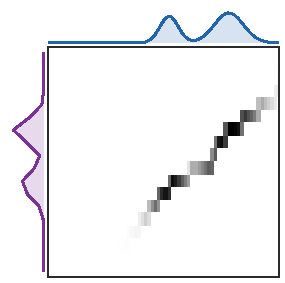
\includegraphics[width=.22\linewidth]{figures/kantorovich-discrete-gluing-lemma/bc-plan.pdf} &
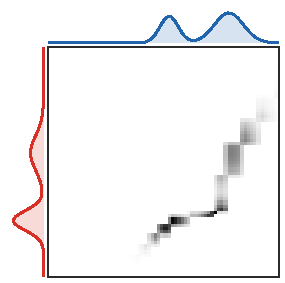
\includegraphics[width=.22\linewidth]{figures/kantorovich-discrete-gluing-lemma/glued-ac-plan.pdf} &
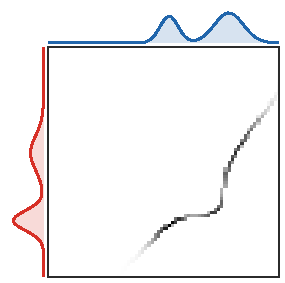
\includegraphics[width=.22\linewidth]{figures/kantorovich-discrete-gluing-lemma/direct-ac-plan.pdf} \\[-.1em]
\small $\a$ to $\b$ &
\small $\b$ to $\c$ &
\small glued $\a$ to $\VectMode{c}$ &
\small direct $\a$ to $\VectMode{c}$
\end{tabular}
\caption{Discrete gluing lemma in matrix form. The first two coupling matrices share the intermediate marginal $\b$. Multiplying through this common marginal gives a feasible glued plan between $\a$ and $\VectMode{c}$, which is the coupling used in the triangle-inequality proof. The last panel shows the direct optimal coupling for comparison.}
\label{fig:kantorovich-discrete-gluing-lemma}
\end{figure}

In one dimension, the geodesic can be read directly in quantile coordinates. Figure~\ref{fig:monge-1d-quantile-geodesic} is the static prototype for the Lagrangian views of one-dimensional PDEs used later in the dynamic and gradient-flow sections.

\begin{figure}[ht]
\centering
\begin{tabular}{@{}ccc@{}}
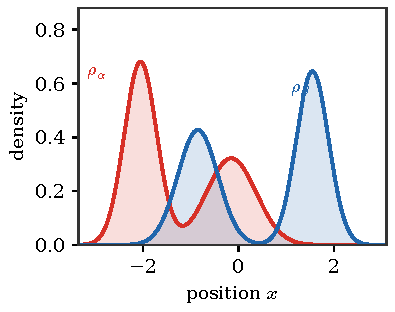
\includegraphics[width=.30\linewidth]{figures/monge-1d-quantile-geodesic/endpoint-densities.pdf} &
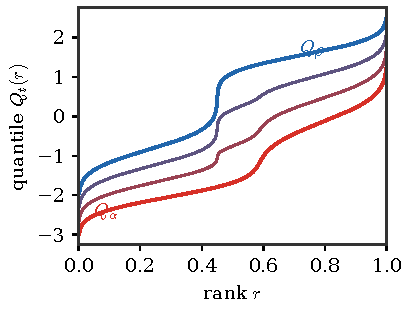
\includegraphics[width=.30\linewidth]{figures/monge-1d-quantile-geodesic/quantiles.pdf} &
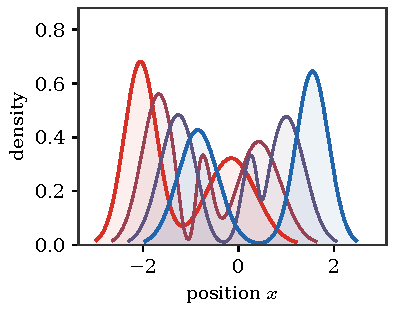
\includegraphics[width=.30\linewidth]{figures/monge-1d-quantile-geodesic/geodesic-densities.pdf} \\[-.1em]
\small endpoint densities &
\small quantile interpolation &
\small geodesic densities
\end{tabular}
\caption{One-dimensional Wasserstein geodesic by quantiles. The optimal coupling matches equal quantile levels, so the interpolation is linear in inverse-CDF coordinates: $Q_t=(1-t)Q_0+tQ_1$. The right panel shows the corresponding density path.}
\label{fig:monge-1d-quantile-geodesic}
\end{figure}

\Needspace{11\baselineskip}
\paragraph{Interpolation induced by an optimal plan.}
\label{sec-kantorovich-plan-interpolation}

For $\X=\RR^d$ and $p=2$, an optimal plan also defines a constant-speed geodesic. If $\pi$ is optimal between $\alpha_0$ and $\alpha_1$, set
\begin{defn}[$\Wass_2$ geodesic induced by an optimal plan]\label{def-w2-geodesic-induced-by-plan}
\begin{equation}\label{eq-plan-interpolation}
	\alpha_t
	=
	((1-t)P_0+tP_1)_\sharp\pi,
	\qquad
	P_0(x,y)=x,
	\quad
	P_1(x,y)=y.
\end{equation}
\end{defn}
When $\pi=(\Id,T)_\sharp\alpha_0$ is induced by a Brenier map, this reduces to McCann's displacement interpolation
\[
	\alpha_t=((1-t)\Id+tT)_\sharp\alpha_0.
\]

\begin{prop}[Optimal-plan interpolation is a $\Wass_2$ geodesic]\label{prop-plan-interpolation-w2-geodesic}
	Let $\pi$ be an optimal coupling between $\alpha_0,\alpha_1\in\Pp_2(\RR^d)$ and define $\alpha_t$ by~\eqref{eq-plan-interpolation}. Then
	\[
		\Wass_2(\alpha_s,\alpha_t)=|t-s|\Wass_2(\alpha_0,\alpha_1),
		\qquad
		0\leq s,t\leq1.
	\]
\end{prop}
\begin{proof}
	Coupling the particles at times $s$ and $t$ through the same endpoint pair $(x,y)\sim\pi$ gives
	\[
		\Wass_2^2(\alpha_s,\alpha_t)
		\leq
		(t-s)^2\int\norm{x-y}^2\,\d\pi
		=
		(t-s)^2\Wass_2^2(\alpha_0,\alpha_1).
	\]
	The reverse inequality follows from the triangle inequality applied to the three pieces $[0,s]$, $[s,t]$ and $[t,1]$.
\end{proof}

The last two primer figures should be read together. Figure~\ref{fig:kantorovich-plan-interpolation} illustrates the definition when the plan is a genuine coupling rather than a single-valued map: each active pair $(x,y)$ follows a straight segment. Figure~\ref{fig:monge-shape-mccann-interpolation} then shows the Monge/Brenier special case on two silhouettes.

\begin{figure}[ht]
\centering
\setlength{\tabcolsep}{1.5pt}
\begin{tabular}{@{}ccccc@{}}
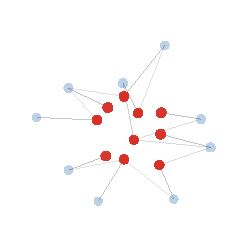
\includegraphics[width=.19\linewidth]{figures/kantorovich-plan-interpolation/time-000.pdf} &
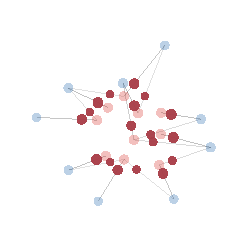
\includegraphics[width=.19\linewidth]{figures/kantorovich-plan-interpolation/time-025.pdf} &
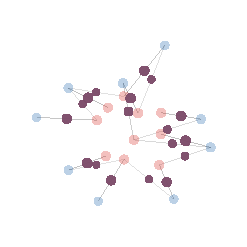
\includegraphics[width=.19\linewidth]{figures/kantorovich-plan-interpolation/time-050.pdf} &
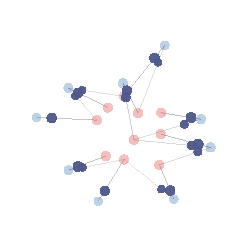
\includegraphics[width=.19\linewidth]{figures/kantorovich-plan-interpolation/time-075.pdf} &
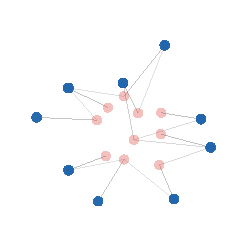
\includegraphics[width=.19\linewidth]{figures/kantorovich-plan-interpolation/time-100.pdf} \\[-.1em]
\small $t=0$ &
\small $t=1/4$ &
\small $t=1/2$ &
\small $t=3/4$ &
\small $t=1$
\end{tabular}
\caption{Interpolation induced by a Kantorovich plan. Each nonzero entry of an optimal discrete coupling transports mass along the segment $(1-t)x_i+ty_j$. This construction is the static plan-level ancestor of the dynamic Benamou--Brenier viewpoint developed in Section~\ref{sec-dynamic-optimal-transport}.}
\label{fig:kantorovich-plan-interpolation}
\end{figure}

\begin{figure}[htbp]
\centering
\begin{tabular}{@{}ccccc@{}}
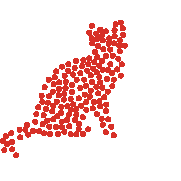
\includegraphics[width=.17\linewidth]{figures/monge-shape-mccann-interpolation/particles-t000.pdf} &
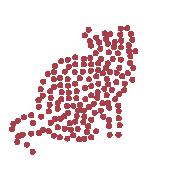
\includegraphics[width=.17\linewidth]{figures/monge-shape-mccann-interpolation/particles-t025.pdf} &
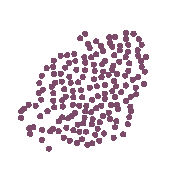
\includegraphics[width=.17\linewidth]{figures/monge-shape-mccann-interpolation/particles-t050.pdf} &
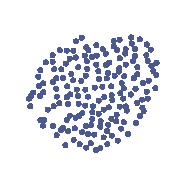
\includegraphics[width=.17\linewidth]{figures/monge-shape-mccann-interpolation/particles-t075.pdf} &
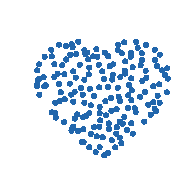
\includegraphics[width=.17\linewidth]{figures/monge-shape-mccann-interpolation/particles-t100.pdf} \\[-.1em]
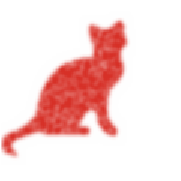
\includegraphics[width=.17\linewidth]{figures/monge-shape-mccann-interpolation/density-t000.pdf} &
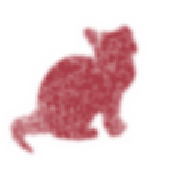
\includegraphics[width=.17\linewidth]{figures/monge-shape-mccann-interpolation/density-t025.pdf} &
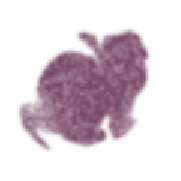
\includegraphics[width=.17\linewidth]{figures/monge-shape-mccann-interpolation/density-t050.pdf} &
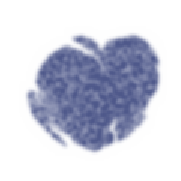
\includegraphics[width=.17\linewidth]{figures/monge-shape-mccann-interpolation/density-t075.pdf} &
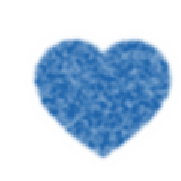
\includegraphics[width=.17\linewidth]{figures/monge-shape-mccann-interpolation/density-t100.pdf} \\[-.1em]
\small $t=0$ & \small $t=1/4$ & \small $t=1/2$ & \small $t=3/4$ & \small $t=1$
\end{tabular}
\caption{McCann displacement interpolation between two silhouette measures. The first row displays transported particles along $T_t(x)=(1-t)x+tT(x)$; the second row renders kernel-smoothed densities from a denser transported cloud. This is the map-induced version of the plan interpolation above and the geometric path used later by Wasserstein gradient-flow arguments.}
\label{fig:monge-shape-mccann-interpolation}
\end{figure}

This geodesic viewpoint is the static counterpart of the Benamou--Brenier formulation in Section~\ref{sec-dynamic-optimal-transport}. It is also the geometry behind the Wasserstein gradient flows of Section~\ref{sec-wasserstein-gradient-flows}.

\FloatBarrier
